
%%%%%%%%%%%%%%%%%%%%%%% file typeinst.tex %%%%%%%%%%%%%%%%%%%%%%%%%
%
% This is the LaTeX source for the instructions to authors using
% the LaTeX document class 'llncs.cls' for contributions to
% the Lecture Notes in Computer Sciences series.
% http://www.springer.com/lncs       Springer Heidelberg 2006/05/04
%
% It may be used as a template for your own input - copy it
% to a new file with a new name and use it as the basis
% for your article.
%
% NB: the document class 'llncs' has its own and detailed documentation, see
% ftp://ftp.springer.de/data/pubftp/pub/tex/latex/llncs/latex2e/llncsdoc.pdf
%
%%%%%%%%%%%%%%%%%%%%%%%%%%%%%%%%%%%%%%%%%%%%%%%%%%%%%%%%%%%%%%%%%%%


\documentclass[runningheads,a4paper]{llncs}

\usepackage{amssymb}
\setcounter{tocdepth}{3}
\usepackage{graphicx}
\usepackage{color}
\usepackage{ulem}
\usepackage{algorithmic}
\usepackage{url}
%\usepackage{amsthm}
\urldef{\mailsa}\path|juliocesar.garcia@caos.uab.es|
%\urldef{\mailsb}\path|anna.kramer, leonie.kunz, christine.reiss, nicole.sator,|
%\urldef{\mailsc}\path|erika.siebert-cole, peter.strasser, lncs}@springer.com|    
\newcommand{\keywords}[1]{\par\addvspace\baselineskip
\noindent\keywordname\enspace\ignorespaces#1}
%\newtheorem{mydef}{Definition}

\begin{document}

\mainmatter  % start of an individual contribution

% first the title is needed
\title{Pseudo Suffix tree to search Maximal Unique Matches between DNA sequences.}

% a short form should be given in case it is too long for the running head
\titlerunning{Pseudo Suffix tree to search Maximal Unique Matches between DNA sequences.}

% the name(s) of the author(s) follow(s) next
%
% NB: Chinese authors should write their first names(s) in front of
% their surnames. This ensures that the names appear correctly in
% the running heads and the author index.
%
\author{Julio C\'esar Garc\'ia Vizca\'ino%
\thanks{}
%\and Antonio Espinosa\and Juan Carlos Moure\and Porfidio Hern\'andez}
%
\authorrunning{Julio C\'esar Garc\'ia Vizca\'ino}
% (feature abused for this document to repeat the title also on left hand pages)

% the affiliations are given next; don't give your e-mail address
% unless you accept that it will be published
\institute{Computer Architecture \& Operating Systems Department (CAOS), Universitat Aut\'onoma de Barcelona,%
    Bellaterra (Barcelona), Spain.
\mailsa\\
%\mailsb\\
%\mailsc\\
\url{http://caos.uab.es}}

%
% NB: a more complex sample for affiliations and the mapping to the
% corresponding authors can be found in the file "llncs.dem"
% (search for the string "\mainmatter" where a contribution starts).
% "llncs.dem" accompanies the document class "llncs.cls".
%

\toctitle{Pseudo Suffix tree to search Maximal Unique Matches between DNA sequences.}
\tocauthor{Julio C\'esar Garc\'ia Vizca\'ino}
\maketitle


\begin{abstract}
  \keywords{}
\end{abstract}


\section{Introduction}
Today, we know that species are described by DNA, a complex molecule comprised of many smaller molecules called nucleotides. The data describing a single specie,commonly called a genome, can be millions or billions of nucleotides long.\\
One of the most basic computational tasks that we perform on genomic data is identifying the evolutionary relationships between DNA from two or more species. On a smaller scale, we wish to identify which individual nucleotides are unique to species, and which nucleotides share ancestry. On a larger scale, we look to \textbf{find entire subsequences that are a common between them}.\\
Currently the availability of a huge amount of  Bioinformatics data (often in the public domain), and on the other hand the  need for new and efficient methods and algorithms capable of  compute the information contained in the data requires to index the Bioinformatics data in order to search on it. As a matter of fact, the  emphasis of research in Bioinformatics and data structures is shifting from the development of data storing and handling methods, to the one of methods able to  extract useful information from data.\\
Consequently, the computational demands needed to explore and analyze the data contained in the genome sequences is quickly becoming a great concern. To meet these demands, we must use data structures to index the genomic data with an important tradeoff between efficient use of memory and CPU resources.\\
This paper focuses in the search of Maximal Unique Matches to make a whole genome alignment. A whole genome alignment is the process of identifying a mapping from each position in query genome to its corresponding position in the reference genome.\\ 
We now describe some notation, give a more detailed introduction to whole genome alignment, and describe the mathematical framework on which we base most of techniques used to perform whole genome alignment. First we define some basic notation. We use R (Reference) and Q (Query) to denote sequences. For sequence R, we refer to position $i$ as $R_{i}$ and let the first position be $R_{0}$.\\
Whole genome alignment is the primary tool for finding evolutionary relationships between DNA sequences. A DNA sequence is a string over four symbols: A, T , C, and G. DNA sequences from individuals of a specie contain many differences. When aligning DNA sequences from different species, large scale changes, such as long insertions and deletions, duplications, reversals and translocations, are common. The goal of whole genome alignment is to infer which changes occurred with a mathematical model that abstracts the physical mutation processes. Finding all these changes is a time-intensive operation in whole genome alignment. Moreover, the size of the genome can be an issue when there is not enough memory to store the reference and query genome.\\
Dynamic programming is too slow for aligning two large genomes. Heuristics such as BLAST \cite{Blast} or FASTA \cite{Fasta} are not designed to perform pairwise alignments of two very long sequences. One very successful approach is based on identifying ``Maximal Unique Matches'', which is based on the assumption that one expects to substrings occurring in two similar genomes. Maximal Unique Matches (MUMs) are almost surely part of a good alignment of the two sequences and so the whole genome alignment problem can be reduced to aligning the genome in the gaps between the MUMs.\\
\begin{quote}
  Given two sequences R, Q $\in \Sigma^*$, and a number $L > 0$. The Maximal Unique Match problem is to find all matches $k \in \Sigma^*$ with
  \begin{itemize}
    \item $|k|\geq L$,
    \item k occurs exactly once in R and once in Q, and
    \item for any character $a \in \Sigma$ neither ka nor ak occurs both in R and Q.
  \end{itemize}
\end{quote}
\section{Related work}
Given the growth of Bioinformatic data nowadays, we require basic string operations over these data such as search operations. Therefore, efficient search algorithms are important components of whole genome alignment. For this reason, specialized data structures like index structures are required in order to speed up string searching. There are many types of index structures. However, we focus in full-text indexes which allow fast access to substrings of any length. Full-text indexes come at a greater memory and construction cost. However, they contain much more information and allow for faster and more flexible search of maximal unique matches. The memory and time performance of many bioinformatic applications are affected by the type and implementation of the index structure used.\\
The three most commonly used full-text index structures in bioinformatics today are suffix trees, suffix arrays and FM-indexes.\\
The suffix tree of a string $S$ contains information about all suffixes of that string and gives access to all prefixes of those suffixes, thus effectively allows fast access to all substrings of the string $S$. The time complexity for matching $k$ patterns of length $m$ to a string of length $n$ is $O(n+km)$, this is the true power of suffix trees. With enough fast memory, suffix trees are likely the best data structure to support string-algorithms. For large-scale applications like whole genome alignment, however, memory consumption really becomes a bottleneck. The size of a suffix tree is quite high i.e. up to 10 \cite{lazy} to 20 times \cite{kurtz} higher than the amount of memory required to store the reference genome.\\
Suffix arrays \cite{sa} are a variant of suffix trees, which are made up of an array containing a permutation of the indexes of string $S$. In terms of performance, Suffix arrays have a lower memory footprint and imporved locality. Suffix arrays can exactly match all occurrences of pattern $P$ in string $S$ in $O(m\log n+|occ(P,S)|)$ time using a binary search.\\
Suffix arrays are not that information-rich compared with suffix trees, but require far less memory. They lack of LCP information, constant time access to children and suffix links, which makes them less fit to tacle more complex string matching problems like search of MUMs. In \cite{abouelhoda} was demonstrated how suffix arrays can be embellished with additional arrays to recover the full expressivity of suffix trees. Enhanced suffix arrays support all operations and traversals on suffix tree using the same time complexity. Array representations generally shows better locality than most standard suffix tree representations. Enhanced suffix arrays occupy about the same amount of memory as regular suffix trees  and are thus equally inapplicable for large strings.\\
FM-indexes \cite{fm} is based in the Burrows-Wheeler transform \cite{bwt} as backward searching method. The space requirement is proportional to and sometimes even smaller than that of the indexed string. All occurrences of pattern $P$ can be located in $O(m+|occ(P,S)|\log n)$ time. FM-indexes combine fast string matching with low memory requirements.\\
Choosing appropiate data structures for implementing the different components of suffix trees forms a basic step in lowering their memory requirements. These components include nodes, edges, edge labels, leaf numbers and suffix links.
\section{The MUM: an heuristic approach}
Although a pair of conserved genes rarely contain the same entire sequence, they share a lot of short common substrings and some of them are indeed unique to this pair of genes. For example the following two sequences, R and Q:\\
\begin{center}
    R=\underline{ac} ga \underline{ctc} a \underline{gctac} t \underline{ggtcagctatt} \underline{acttaccgc}\$\\
      Q=\underline{ac} tt \underline{ctc} t \underline{gctac} \underline{ggtcagctatt} c \underline{acttaccgc}\$\\
\end{center}
It is clear that sequences R and Q have many common substrings, they are: ac, ctc, gctac, ggtcagctatt and acttaccgc. Among those five common substrings, ac is the only substring that is not unique. It occurs more than once in both sequences. You can also observe that actually a, c, t, and g are common substrings of R and Q. However, they are not maximal, i.e. they are contained in at least one longer common substrings. We are only interested in those that are unique and of maximal length. For example, assuming d = 3, sequences R and Q in the previous example has four MUMs: ctc, gctac, ggtcagctatt, acttaccgc. Substring ac is not an MUM because its length is smaller than the value of d and it is not unique to both sequences.\\
Our aim is to search for all these short common substrings. Given genomes R and Q, we need to find all common substrings which are unique and of maximal length. Each of such common substrings is known as Maximum Unique Match (MUM). For almost every conserved gene pairs, there exist at least one MUM which is unique to them. {\textbf The concept of MUM is important in whole genome alignment because a significantly long MUM is very likely to be part of the global alignment.}
\subsubsection{Search MUMs in a suffix tree} 
The key idea in this method is to build a suffix tree for genome R, a data structure which allows finding all distinct subsequences in a given sequence. The MUM search algorithm consists of three steps, they are as follows:
\begin{algorithmic}
  \STATE{Build a suffix tree for R}
  \FOR{Every suffix of Q}
  \STATE{Compare it by traversing the suffix tree of R}
  \STATE{Mark every edge found in common between R and Q}
  \STATE{For each marked path, suppose it represents the i-th suffix of R and the j-th suffix of Q.}
  \IF{$R[i-1]\neq Q[j-1]$ and Match is in a leaf node}
  \STATE{The path label of this marked node is a MUM}
  \ENDIF
  \ENDFOR
\end{algorithmic}
\subsubsection{Complexity analysis} 
\begin{itemize}
  \item \textbf{Step 1:} Building a suffix tree can be done in $O(n)$ time \cite{kurtz}.
  \item \textbf{Step 2:} Marking internal nodes takes $O(n)$ time. 
  \item \textbf{Step 3:} Comparing R[i-1] and Q[i-1] for each marked nodes takes $O(n+m)$ time as the number of marked nodes is at most $n+m-2$. By the same reasoning, traversing all internal nodes to extracting MUMs also takes $(n+m)$ time.
  \item In total,this algorithm takes $O(n+m)$ time to find all MUMs of the input sequences.
  \item The space complexity of this method is $O\left(n\log n\right)$ bits as we need to store the suffix tree of the input sequence.
\end{itemize}
Based on some experiments, it is found that MUMs can cover 100\% of the known conserved gene pairs. Moreover, finding all MUMs can be done in linear time.
\section{Pseudo Suffix Tree}
A full-text index data structure is used to solve string-matching problems but when we focus in the search of Maximal Unique Matches then we require to make some observations of the properties of these full-text index data structures. A Maximal Unique Match is unique between a reference and query genome, so that we need to quickly get the uniqueness property in the reference and query genome. Since a reference genome is usually indexed by the data structure we may check which classic full-text index data structure is suitable for this task:
\begin{itemize}
  \item Suffix array: It performs a binary search until a unique match is found.
  \item Suffix tree: It performs a traversal in suffix tree until it reaches a leaf node, this means a unique match in the whole string.
  \item FM-index: It performs a backward search until a unique match is found.
\end{itemize}
Since we are searching for maximal and unique matches the suffix tree is the ideal data structure to do this kind of job. However, the space requirements are prohibitive when handling large genomes. Again the trade-off between time and space performance is a feature desired to find a suitable data structure. As we pointed out a unique match is easily found in a suffix tree because we only require to check if the match is in a leaf node.\\
Therefore, we propose a new full-text index data structure a Pseudo Suffix Tree. The Pseudo Suffix Tree is build based on the information of a Suffix Tree. This data structure has three components: Direct access table, set of suffixes with common prefix order by length and set of suffixes with a common prefix and a fixed length, see Figure \ref{fig:pseudo}.
\begin{figure}
\centering
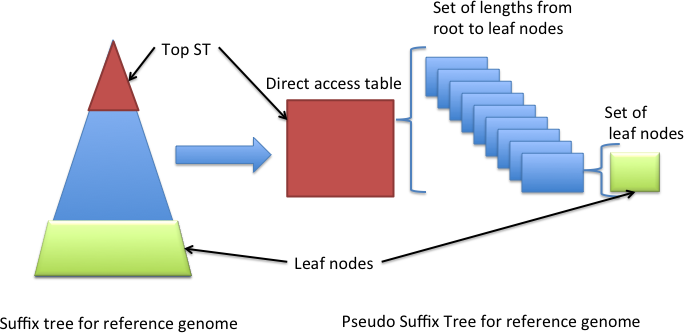
\includegraphics[scale=0.5]{pseudoST.png}
\label{fig:pseudo}
\caption{Pseudo Suffix Tree for a reference genome to search Maximal Unique Matches.}
\end{figure}
\subsection{Direct access table}
A Direct access table contains a set of prefixes of a fixed length $P$ from the top of the suffix tree, see Figure \ref{fig:dat}. This table has entries in the form of an 2-bit encoding string of DNA (a:00,c:01,g:10,t:11) so that we can access in $O(1)$ to any element of this table with an encoded string to an integer. For instance, if we defined a fixed length of $P=2$ we have entries in the table from 0 to $4^2$. where aa would be saved as 0 and tt would be saved as 15.\\
We require this Direct access table because for every suffix in the query genome we need to check the match from the root of suffix tree. With this table we saved for comparisons and because $P$ has to be small in order to be fast so that it can be cached in the processor.\\
The 2-bit encoding string saved in the Direct access table is the key to access to the value of this table. The value of every entry is a pointer to a set of suffixes with the common prefix in the key of the Direct access table. Therefore the key ac, which is encoded as 1, will have all the suffixes with the common prefix ac.
\begin{figure}
\centering
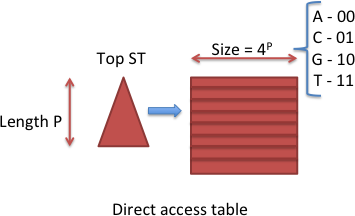
\includegraphics[scale=0.5]{DAT.png}
\label{fig:dat}
\caption{Direct Access Table with 2-bit encoding DNA for a reference genome to search Maximal Unique Matches.}
\end{figure}
\subsection{Set of suffixes with a length to leaf nodes}
The value of the Direct access table is a set of suffixes with a common prefix, see Figure \ref{fig:depth}. We need to store this suffixes because we are interested in the search of unique matches. To check if we have a unique match we need to reach a leaf node. The leaf node in a Suffix tree stores the position in the reference genome where the suffix starts and to save space the depth of the leaf node indicates the number of characters from the root until the leaf node which is the path inside the Suffix tree for this suffix. This depth in the leaf node allows us to continue reading the suffix until a mismatch occurs. The key in this table is the length to leaf nodes and the value is the list of suffixes.
\begin{figure}
\centering
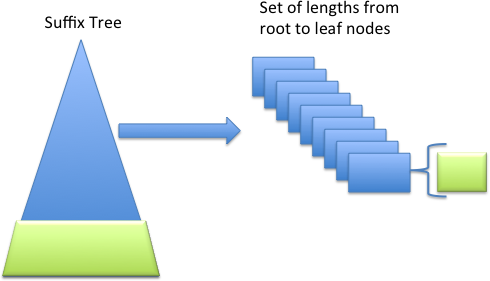
\includegraphics[scale=0.5]{Depth.png}
\label{fig:depth}
\caption{Set of suffixes with a length to leaf nodes for a reference genome to search Maximal Unique Matches.}
\end{figure}
\subsection{Set of suffixes with a fixed length}
Every suffix has a depth until the leaf node, so that we have a set of suffixes which have a common prefix in the Direct access table and with a fixed length from the root of suffix tree. We group the suffixes in this way because we are interested only in the search of MUMs, see Figure \ref{fig:suffixes}.
\begin{figure}
\centering
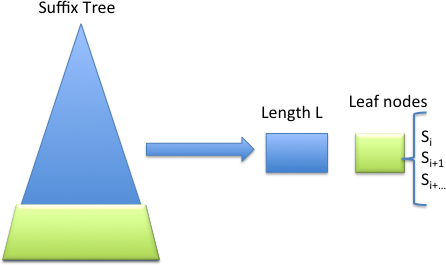
\includegraphics[scale=0.5]{Leaf.png}
\label{fig:suffixes}
\caption{List of leaf nodes with suffix start position for a reference genome to search Maximal Unique Matches.}
\end{figure}
\section{Search of Maximal Unique Matches in Pseudo Suffix Tree}
The search of MUMs in a Suffix Tree requires the traversal of Suffix Tree from the root until the leaf node for every suffix in the query genome. We may improve the search of MUMs by using suffix links, therefore we do not need to go back to root with every new suffix in the query genome.  However, with huge Suffix Tree this improvement involves a high random access to the data structure in main memory. \\
With our proposal of a Pseudo Suffix Tree we apply an heuristic to search MUMs: only to check those suffixes with a match in the leaf nodes of a Suffix Tree. Because our Pseudo Suffix Tree stores the length of the suffixes where the leaf node starts, we may check if the match is long enough to reach the leaf node and quickly discard those suffixes in the query which are not long enough to reach a leaf node.\\
In the Figure \ref{fig:algo} is shown the search for some suffix starting in position of Query genome, $Q_{i}$. We encoded the prefix of size $P$ and search the entry in the Direct Access Table in order to get the list of suffixes to search for MUMs. For every length in this set we require to check if this match is maximal with the current suffix in reference $j$, to test this feature we evaluate if $R_{j-1}!=Q_{i-1}$ and $R_{j+length+1}==Q_{i+length+1}$ is true. Then we only have to evaluate the longest common prefix between the subset of suffixes in Reference and the current suffix in Query. \\
\begin{figure}
\centering
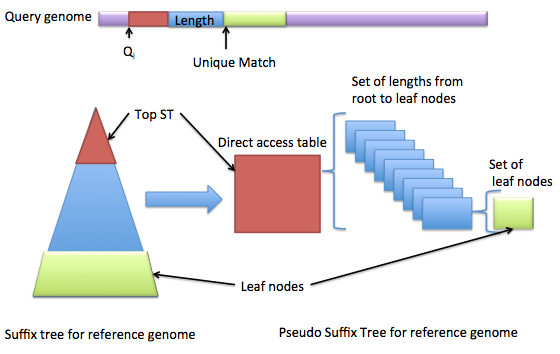
\includegraphics[scale=0.5]{pseudost-mum.png}
\label{fig:algo}
\caption{Set of suffixes with a length to leaf nodes for a reference genome to search Maximal Unique Matches.}
\end{figure}
After we have read the Query, we have a list of MUM candidates. A MUM candidate is a match which is unique in the Reference genome but it may not be in the Query genome. This feature is shown in Figure \ref{fig:mumcand}, where a MUM candidate is found while reading the Query and after some suffixes a new MUM candidate is found with the same match in the Reference genome.
\begin{figure}
\centering
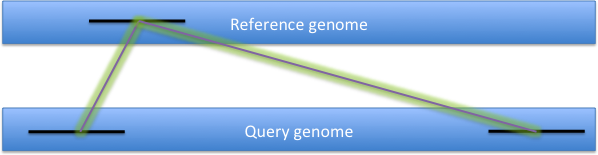
\includegraphics[scale=0.5]{Whole-MUM.png}
\label{fig:mumcand}
\caption{MUM candidates that are not a real MUM.}
\end{figure}
We drop these MUM candidates and we finally have a list of real MUMs with the following information: start position in Reference genome, start position in Query genome and length of MUM.
\section{Implementation \& Results}
Our main objective is to find Maximal Unique Matches and we evaluated how useful is our Pseudo Suffix Tree to search MUMs. We measure the access to the subset of suffixes which should be searched for MUMs for several lengths of the Direct Access Table. Our set of genomes were: 1kbp\footnote{bp is base pair and is the basic unit measure for genome data.}, 10kbp, 100kbp and a real genome (EcoliK12 and EcoliO157H7) of about 5Mbp.\\
Our implementation is based on associative containers, the type used is map from the C++ language. The Direct Access Table is map because it allows a direct access of the mapped valued. The key is the 2-bit encoded string of the prefix and the value is the set of suffixes with the common prefix. The set of suffixes is also a map which has the key as the length until the leaf node in the Suffix Tree and the value is a vector with the list of suffixes with the same length. In this way we can access to any suffix with a common prefix and a required length. Although the map container allows a direct access to the elements of the Pseudo Suffix Tree, these map containers are implemented as a red black tree. The main consequence is logarithmic complexity for insertion and search.\\
In Figures \ref{fig:1k,fig:10k,fig:100k} we show that a short length for the Direct Access Table requires to check more suffixes. When we increase the length of the common prefix we reduce the set of suffixes to search. In Figure \ref{fig:ecoli} we show that with a real genome the reduced subset of suffixes to search for is small enough compared with a naive solution. With a larger length in the Direct Access Table we reduced the set of suffixes to search from 31\% with a length of 11bp to 0.1\% with a length of 16bp.\\
\begin{figure}
\centering
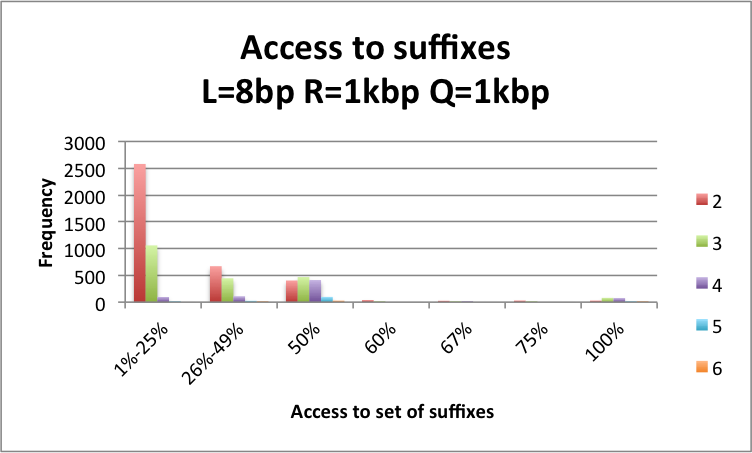
\includegraphics[scale=0.5]{1k.png}
\label{fig:1k}
\caption{Different lengths for Direct Access Table.}
\end{figure} 
\begin{figure}
\centering
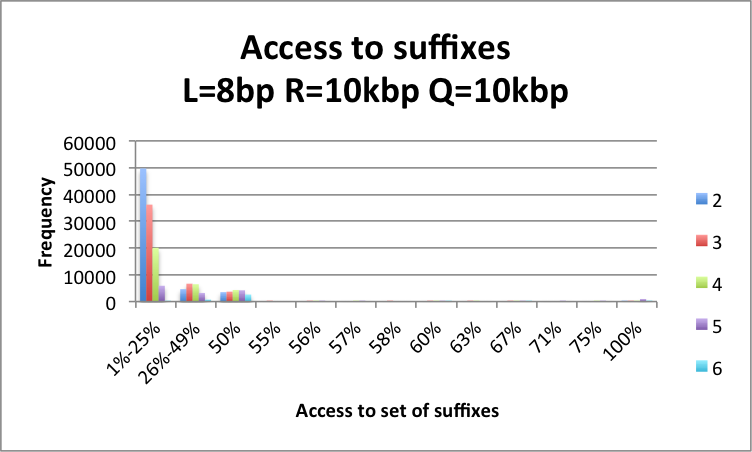
\includegraphics[scale=0.5]{10k.png}
\label{fig:10k}
\caption{Different lengths for Direct Access Table.}
\end{figure}
\begin{figure}
\centering
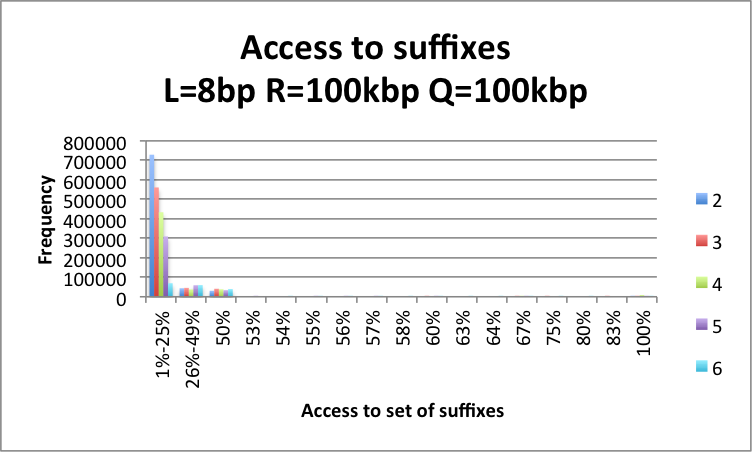
\includegraphics[scale=0.5]{100k.png}
\label{fig:100k}
\caption{Different lengths for Direct Access Table.}
\end{figure}
\begin{figure}
\centering
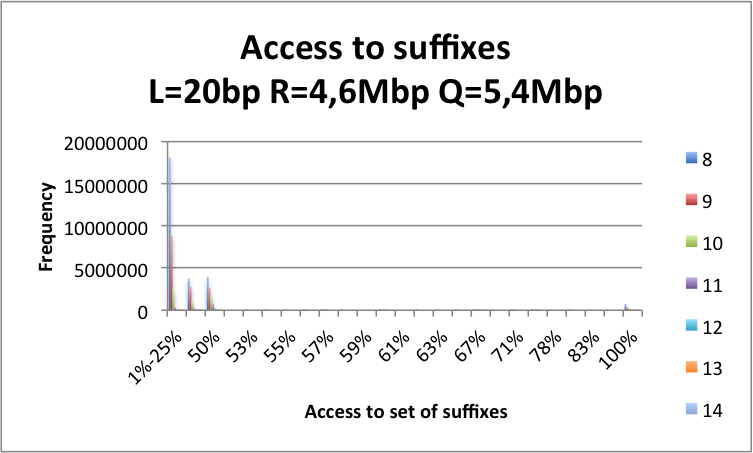
\includegraphics[scale=0.5]{Ecoli.png}
\label{fig:ecoli}
\caption{Different lengths for Direct Access Table.}
\end{figure}
We also measured the access to the Pseudo Suffix Tree to search for MUMs, in Figure \ref{fig:pst} we show that Pseudo Suffix Tree is extremely slow. This is because we have to check for the whole set of suffixes for every suffix in the query genome.
\begin{figure}
\centering
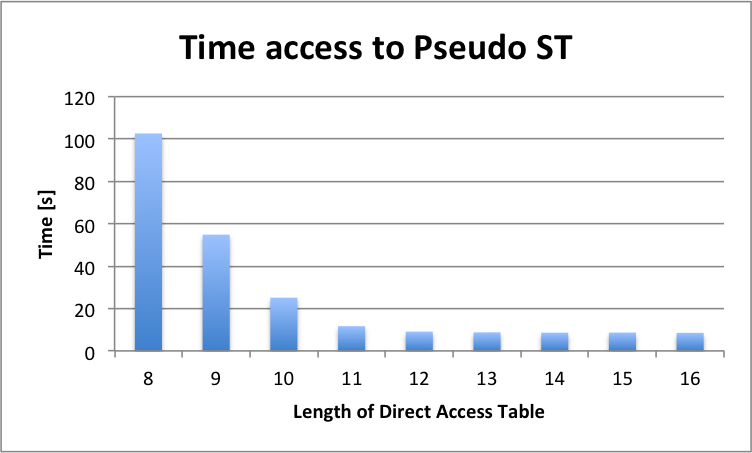
\includegraphics[scale=0.5]{time.png}
\label{fig:pst}
\caption{Access time to get Suffixes in Pseudo Suffix Tree for Ecoli genome.}
\end{figure}
\begin{thebibliography}{8}
  \bibitem{Blast} Altschul, S. F. and Gish, W. and Miller, W. and Myers, E. W. and Lipman, D. J.: Basic local alignment search tool. J. Mol. Biol. 215, 403--410 (1990)
  \bibitem{Fasta} D. J. Lipman, W. R. Pearson: Rapid and sensitive protein similarity searches. Science (New York, N.Y.), Vol. 227, No. 4693. (22 March 1985), pp. 1435-1441.
  \bibitem{lazy} Giegerich, R., S. Kurtz, and J. Stoye.: Efficient implementation of lazy suffix trees. Softw. Pract. Exper 33 (2003): 1035-1049.
  \bibitem{kurtz} S. Kurtz: Reducing the space requirement of suffix trees. Software: Practice and Experience, Vol. 29, No. 13. (November 1999), pp. 1149-1171.
  \bibitem{abouelhoda} Abouelhoda, M. I., Kurtz, S., \& Ohlebusch, E.: Replacing suffix trees with enhanced suffix arrays. (2004) Journal of Discrete Algorithms, 2(1).
  \bibitem{fm} Ferragina, P., and Manzini, G.: Opportunistic data structures with applications. In Proceedings of the 41st IEEE Symposium on Foundations of Computer Science. Redondo Beach, California, USA. pp. 390-398.
  \bibitem{bwt} Burrows, M., and Wheeler, D.J.: A block-sorting lossless data compression algorithm. Technical report, Digital SRC, Research Report 124, 10 May 1994.
  \bibitem{sa} Manber, U, and Myers, E.: Suffix arrays: a new method for on-line string searches. SIAM J. Comput., 22, 935-948.
\end{thebibliography}

\end{document}
